
\documentclass[border=10pt, 12pt]{standalone}
\usepackage[svgnames]{xcolor}
\usepackage{amsmath}
\usepackage{pgfplots}
\pgfplotsset{compat=newest}
\usepackage[sfdefault]{FiraSans}
\usepackage{FiraMono}
\renewcommand*\familydefault{\sfdefault}
\begin{document}
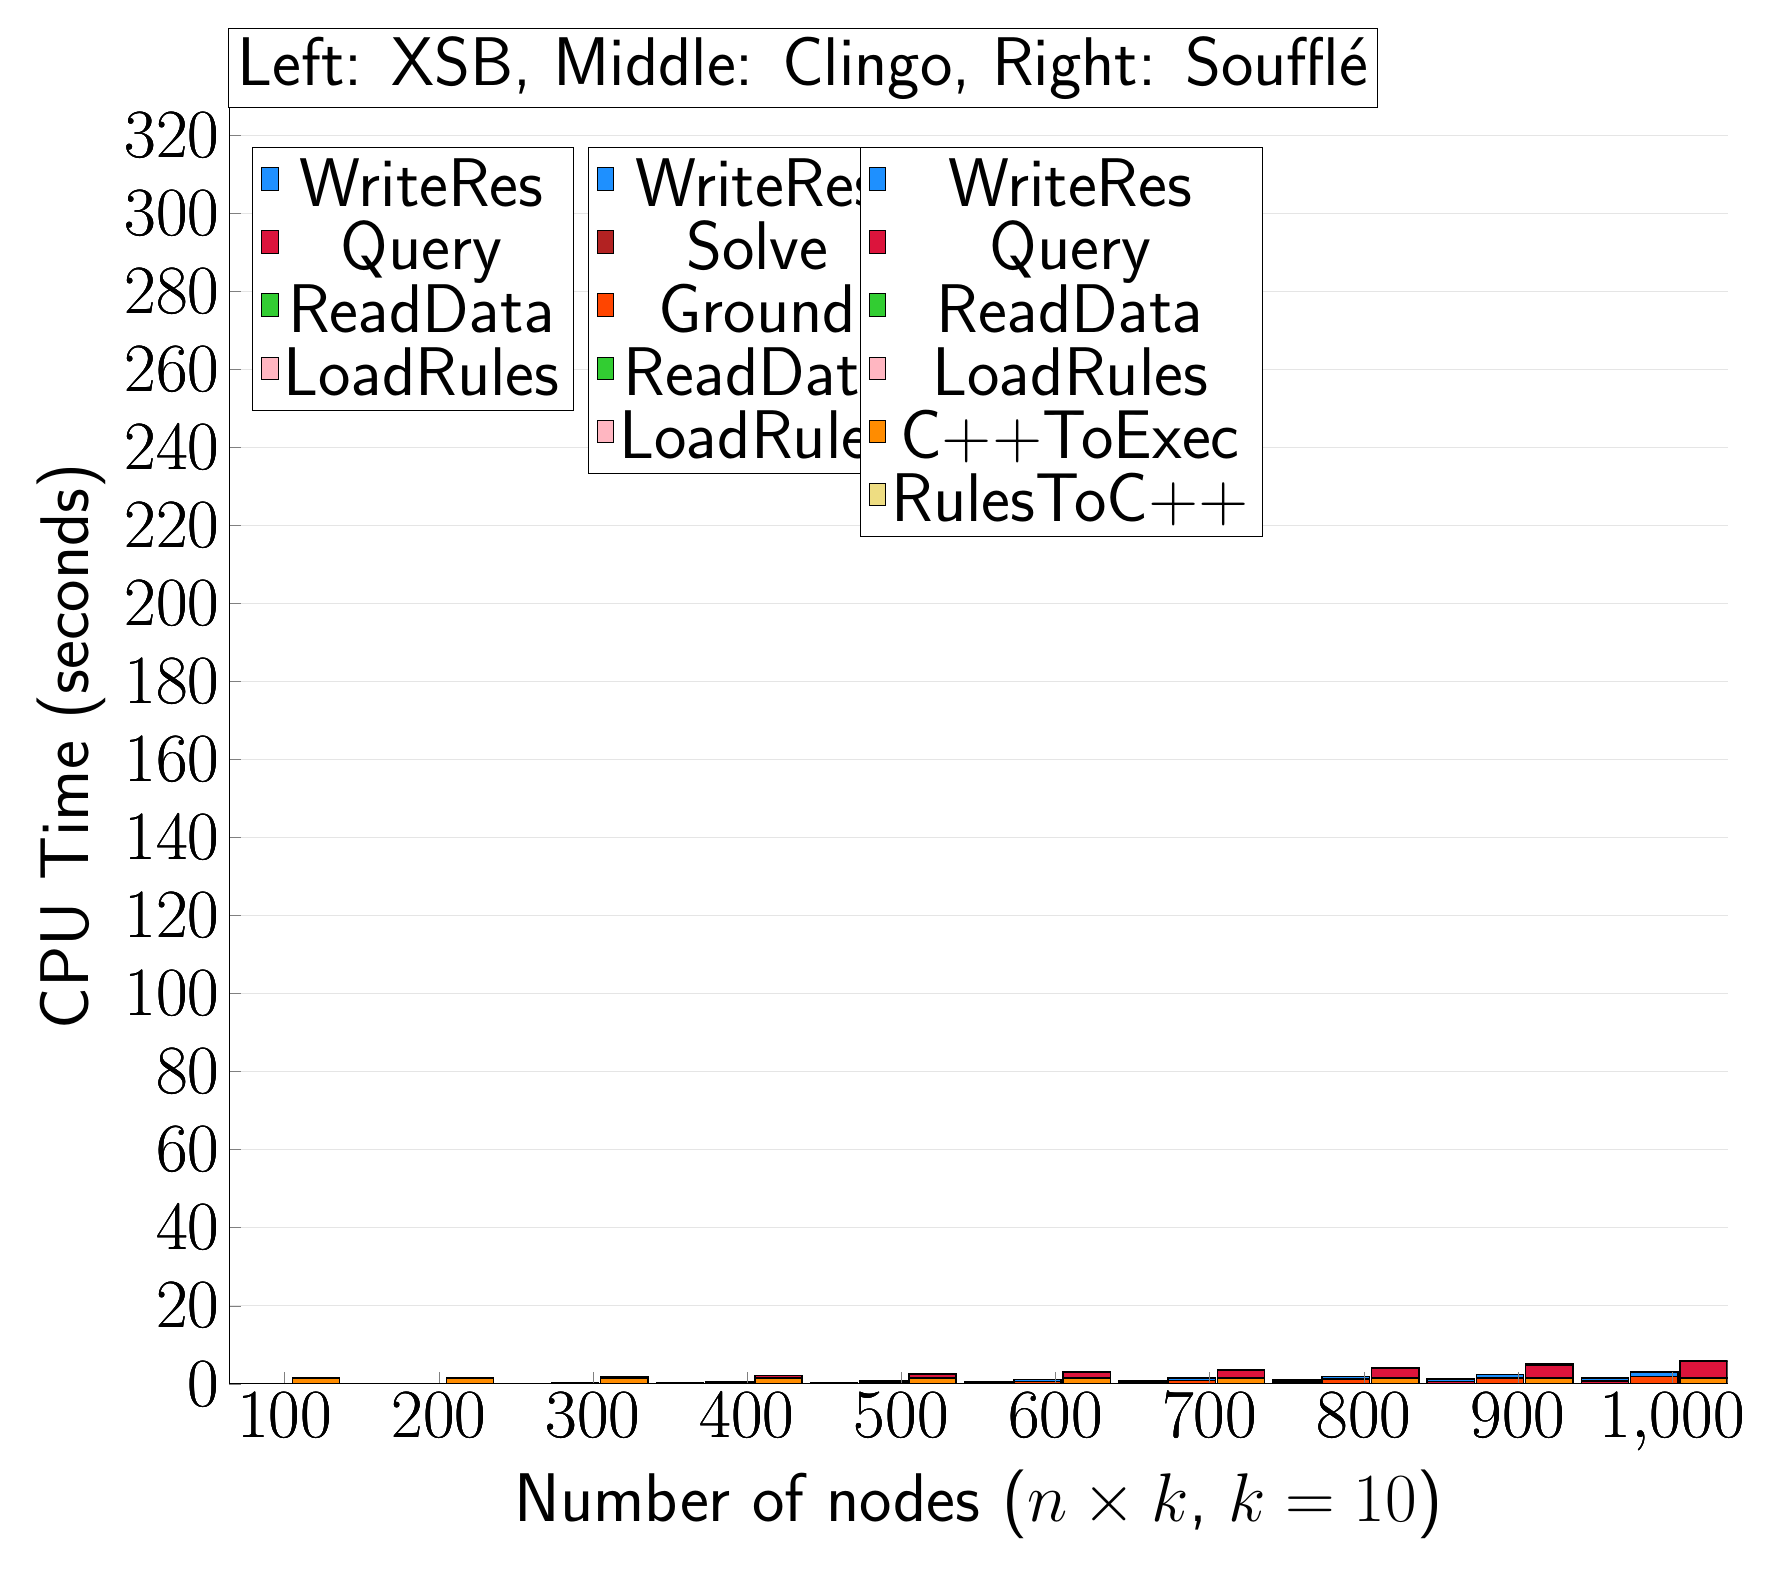
\begin{tikzpicture}
                        \begin{axis}[bar shift=-24.3pt, 
   ybar stacked,
   width=1.7\textwidth,
   bar width=0.6cm,
   ymajorgrids, tick align=inside,
   major grid style={draw=gray!20},
   xtick=data,
   ymin=0, ymax=326.9108,
   axis x line*=bottom,
   axis y line*=left,
   enlarge x limits=0.04,
   legend style={
       at={(0.23, 0.97)},
       anchor=north east,
       legend columns=1,
       font=\Huge,
   },
   ylabel={CPU Time (seconds)},
   xlabel={Number of nodes ($n \times k$, $k=10$)},
   label style={font=\Huge},
   tick label style={font=\Huge},
]
\addlegendimage{fill=DodgerBlue, draw=black, line width=0.2pt}
\addlegendentry{WriteRes}
\addlegendimage{fill=Crimson, draw=black, line width=0.2pt}
\addlegendentry{Query}
\addlegendimage{fill=LimeGreen, draw=black, line width=0.2pt}
\addlegendentry{ReadData}
\addlegendimage{fill=LightPink, draw=black, line width=0.2pt}
\addlegendentry{LoadRules}
\addplot +[fill=LightPink, draw=black, line width=0.55pt] coordinates {
(100, 0.0005503999999999997)
(200, 0.0005548)
(300, 0.0005550000000000004)
(400, 0.0005548)
(500, 0.0005598000000000003)
(600, 0.0005502)
(700, 0.0005549999999999997)
(800, 0.000552)
(900, 0.0005522)
(1000, 0.0005534000000000002)
};
\addplot +[fill=LimeGreen, draw=black, line width=0.55pt] coordinates {
(100, 0.0009649999999999997)
(200, 0.0018515999999999997)
(300, 0.002715)
(400, 0.0035554000000000002)
(500, 0.0044226)
(600, 0.005325)
(700, 0.0062294)
(800, 0.007165200000000001)
(900, 0.007933399999999998)
(1000, 0.008800200000000001)
};
\addplot +[fill=Crimson, draw=black, line width=0.55pt] coordinates {
(100, 0.006647600000000001)
(200, 0.028298200000000003)
(300, 0.06300460000000001)
(400, 0.1113696)
(500, 0.1786858)
(600, 0.2549788)
(700, 0.34303999999999996)
(800, 0.4442016)
(900, 0.6097274)
(1000, 0.7310082)
};
\addplot +[fill=DodgerBlue, draw=black, line width=0.55pt] coordinates {
(100, 0.008199000000000001)
(200, 0.032584)
(300, 0.072255)
(400, 0.1281278)
(500, 0.2009166)
(600, 0.2807278)
(700, 0.3955704)
(800, 0.513282)
(900, 0.6481910000000001)
(1000, 0.7921046)
};
\end{axis}

\begin{axis}[bar shift=-6.5pt, 
   ybar stacked,
   width=1.7\textwidth,
   bar width=0.6cm,
   ymajorgrids, tick align=inside,
   major grid style={draw=none},
   xtick=data,
   ymin=0, ymax=326.9108,
   axis x line*=none,
   axis y line*=none,
   enlarge x limits=0.04,
   legend style={
       at={(0.454, 0.97)},
       anchor=north east,
       legend columns=1,
       font=\Huge,
   },
   label style={font=\Huge},
   tick label style={font=\Huge},
]
\addlegendimage{fill=DodgerBlue, draw=black, line width=0.2pt}
\addlegendentry{WriteRes}
\addlegendimage{fill=FireBrick, draw=black, line width=0.2pt}
\addlegendentry{Solve}
\addlegendimage{fill=OrangeRed, draw=black, line width=0.2pt}
\addlegendentry{Ground}
\addlegendimage{fill=LimeGreen, draw=black, line width=0.2pt}
\addlegendentry{ReadData}
\addlegendimage{fill=LightPink, draw=black, line width=0.2pt}
\addlegendentry{LoadRules}
\addplot +[fill=LightPink, draw=black, line width=0.55pt] coordinates {
(100, 0.0)
(200, 0.0)
(300, 0.0)
(400, 0.0)
(500, 0.0)
(600, 0.0)
(700, 0.0)
(800, 0.0)
(900, 0.0)
(1000, 0.0)
};
\addplot +[fill=LimeGreen, draw=black, line width=0.55pt] coordinates {
(100, 0.0)
(200, 0.0)
(300, 0.0040000000000000036)
(400, 0.010000000000000009)
(500, 0.010000000000000009)
(600, 0.01200000000000001)
(700, 0.010000000000000009)
(800, 0.020000000000000018)
(900, 0.020000000000000018)
(1000, 0.020000000000000018)
};
\addplot +[fill=OrangeRed, draw=black, line width=0.55pt] coordinates {
(100, 0.020000000000000018)
(200, 0.062)
(300, 0.14400000000000002)
(400, 0.252)
(500, 0.4080000000000001)
(600, 0.606)
(700, 0.8460000000000001)
(800, 1.108)
(900, 1.4259999999999997)
(1000, 1.802)
};
\addplot +[fill=FireBrick, draw=black, line width=0.55pt] coordinates {
(100, 0.0)
(200, 0.006000000000000005)
(300, 0.0020000000000000018)
(400, 0.012000000000000009)
(500, 0.020000000000000018)
(600, 0.020000000000000018)
(700, 0.02600000000000003)
(800, 0.041999999999999815)
(900, 0.05800000000000004)
(1000, 0.062000000000000055)
};
\addplot +[fill=DodgerBlue, draw=black, line width=0.55pt] coordinates {
(100, 0.010000000000000009)
(200, 0.03999999999999998)
(300, 0.118)
(400, 0.17999999999999994)
(500, 0.2779999999999999)
(600, 0.4200000000000001)
(700, 0.5699999999999998)
(800, 0.7400000000000002)
(900, 0.916)
(1000, 1.1560000000000001)
};
\end{axis}

\begin{axis}[bar shift=11.3pt, 
   ybar stacked,
   width=1.7\textwidth,
   bar width=0.6cm,
   ymajorgrids, tick align=inside,
   major grid style={draw=none},
   xtick=data,
   ymin=0, ymax=326.9108,
   axis x line*=none,
   axis y line*=none,
   enlarge x limits=0.04,
   legend style={
       at={(0.69, 0.97)},
       anchor=north east,
       legend columns=1,
       font=\Huge,
   },
   label style={font=\Huge},
   tick label style={font=\Huge},
]
\addlegendimage{fill=DodgerBlue, draw=black, line width=0.2pt}
\addlegendentry{WriteRes}
\addlegendimage{fill=Crimson, draw=black, line width=0.2pt}
\addlegendentry{Query}
\addlegendimage{fill=LimeGreen, draw=black, line width=0.2pt}
\addlegendentry{ReadData}
\addlegendimage{fill=LightPink, draw=black, line width=0.2pt}
\addlegendentry{LoadRules}
\addlegendimage{fill=DarkOrange, draw=black, line width=0.2pt}
\addlegendentry{C++ToExec}
\addlegendimage{fill=LightGoldenrod, draw=black, line width=0.2pt}
\addlegendentry{RulesToC++}
\addplot +[fill=LightGoldenrod, draw=black, line width=0.55pt] coordinates {
(100, 0.004000000000000001)
(200, 0.006000000000000001)
(300, 0.008000000000000002)
(400, 0.006000000000000001)
(500, 0.010000000000000002)
(600, 0.006000000000000001)
(700, 0.0020000000000000005)
(800, 0.006000000000000001)
(900, 0.0020000000000000005)
(1000, 0.004000000000000001)
};
\addplot +[fill=DarkOrange, draw=black, line width=0.55pt] coordinates {
(100, 1.482)
(200, 1.482)
(300, 1.4520000000000002)
(400, 1.4540000000000002)
(500, 1.4520000000000004)
(600, 1.47)
(700, 1.4679999999999997)
(800, 1.4480000000000002)
(900, 1.472)
(1000, 1.4780000000000002)
};
\addplot +[fill=LightPink, draw=black, line width=0.55pt] coordinates {
(100, 0.0001464)
(200, 0.000153)
(300, 9.8e-05)
(400, 4.78e-05)
(500, 0.00011800000000000001)
(600, 0.00017959999999999997)
(700, 0.0001672)
(800, 0.0001454)
(900, 0.000149)
(1000, 0.0001656)
};
\addplot +[fill=LimeGreen, draw=black, line width=0.55pt] coordinates {
(100, 0.0043524)
(200, 0.0078052)
(300, 0.0071806)
(400, 0.008126600000000001)
(500, 0.013594400000000001)
(600, 0.020339199999999998)
(700, 0.0212142)
(800, 0.0206714)
(900, 0.0251372)
(1000, 0.028243399999999995)
};
\addplot +[fill=Crimson, draw=black, line width=0.55pt] coordinates {
(100, 0.050414)
(200, 0.1532508)
(300, 0.32878299999999994)
(400, 0.6108724000000001)
(500, 0.9566014)
(600, 1.4009440000000002)
(700, 1.9211940000000003)
(800, 2.554812)
(900, 3.3841900000000003)
(1000, 4.233051999999999)
};
\addplot +[fill=DodgerBlue, draw=black, line width=0.55pt] coordinates {
(100, 0.0027549999999999996)
(200, 0.0088114)
(300, 0.0198364)
(400, 0.034567600000000004)
(500, 0.05414100000000001)
(600, 0.0772374)
(700, 0.10429379999999999)
(800, 0.1370336)
(900, 0.1755298)
(1000, 0.212608)
};
\end{axis}


\node[anchor=south, draw, fill=white] at (rel axis cs:0.42, 1) {\Huge Left: XSB, Middle: Clingo, Right: Soufflé};
\end{tikzpicture}
\end{document}
                    